\section{Support Vector Machines (SVM)}
\subsection{Hard Margin SVM}
\textit{Classification:} given a training set $TR = <x_i,d_i>, \, i=1 \dots N$, find a hyperplane $w^T x + b = 0$ to separate the examples:
\begin{equation}
d_i = \overbrace{sign(g(x))}^{\textbf{Hypothesis}}=
\begin{cases}
+1 & \text{if }    (g(x_i) = w^T x_i + \overbrace{b}^\textbf{bias} )\geq 0 \\
-1 & \text{if }    (\underbrace{g(x_i) = w^T x_i + b )}_{\textbf{Discriminant function}}< 0
\end{cases}
\end{equation}
SVMs find the optimal hyperplane that maximizes the margin between classes, which lowers the generalization error. The \textbf{margin} $\rho$ is the width of the band around the decision boundary, twice the distance from the hyperplane to the nearest data point. The optimal hyperplane $w_o^Tx + b_o = 0$ maximizes this margin, with $\rho = 2 / \|w_o\|$ (the \textbf{Maximal Margin Classifier}). We can rescale $w$ and $b$ so the closest points to the separating hyperplane satisfy $|g(x)| = 1$:
\begin{equation}\label{SVMresclaed}
d_i = \begin{cases}
    +1 & \text{if }w^T x_i + b \geq +1 \\
    -1 & \text{if }w^T x_i + b \leq -1 
\end{cases}    \qquad \overset{compact form}{\Longrightarrow}\qquad     d_i(w^T x_i + b) \geq 1
\end{equation}
\begin{itemize}
    \item \textbf{Support vector $x^{(s)}$}: any point $x_i$ satisfying (\ref{SVMresclaed})
\end{itemize}
Let $r$ be the distance between the optimal hyperplane and $x = x_p + r\frac{w_o}{\|w_o\|}$ (with \textit{$x_p$ on the hyperplane})
\begin{equation}
    g\left(x_p + r\dfrac{w_o}{\|w_o\|}\right) = g(x_p) + r \dfrac{w_o^T w_o}{\|w_o\|} = r \dfrac{\|w_o\|^2}{\|w_o\|} = r \|w_o\| \Rightarrow r = \dfrac{g(x)}{\|w_o\|}
\end{equation}
For a positive support vector $x^{(s)}$, the distance $r$ equals:
\begin{equation}
    r = \dfrac{g(x^{(s)})}{\|w_o\|} = \dfrac{1}{\|w_o\|} = \dfrac{\rho}{2} \qquad \Longrightarrow \qquad \rho = \dfrac{2}{\|w_o\|}
\end{equation}

\subsubsection{Primal Problem}

The optimal hyperplane maximizes \(\rho\) and minimizes \(\|w\|\). Gradient descent can be used to find \(w\) and \(b\) that achieve these goals.
\paragraph{Quadratic Optimization Problem (Primal Form)}
Given the training examples $TR = < x_i,d_i >$, find:
\begin{equation}
\begin{aligned}
    \min_{w,b} \quad & \Psi(w) = \dfrac{1}{2} w^T w = \dfrac{1}{2} \|w\|^2 \\
    \text{subject to} \quad & d_i (w^T x_i + b) \geq 1, \quad \forall i
\end{aligned}
\end{equation}
\begin{itemize}
    \item $\Psi (w)$ \textit{quadratic} and \textit{convex} in $w$ and constraints are linear in $w$;
    \item solving the problem scales with the size of the input space $m$.
\end{itemize}
\paragraph{How to Solve (Lagrangian Multipliers)}
\begin{equation}
    J(w,b,\lambda) = \dfrac{1}{2}w^T w - \sum_{i=1}^N \lambda_i(d_i(w^T x_i + b) - 1) \quad \lambda_i \geq 0 \textit{ Lagrangian multipliers}
\end{equation}
Each term in the sum is a constraint of the primal problem: $J$ must be minimized with respect to $w$ and $b$ and maximized with respect to $\lambda$. The solution is a saddle point of $J$.

\begin{itemize}
    \item [1.] \textbf{Minimize $J$ with respect to $w$}
    \begin{equation*}
    \dfrac{\partial J}{\partial w} = \dfrac{2}{2} w - \sum_{i=1}^N \lambda_i(d_i(1*x_i + 0) + 0) 
    = w - \sum_{i=1}^N \lambda_i(d_i(x_i)) = 0 \Rightarrow
    w = \sum_{i=1}^N \lambda_i(d_i(x_i))
\end{equation*}
Thus the optimal hyperplane is expressed as:
\begin{equation*}
    g(x) = w_o^T x + b_o = 0 \,\,
    \iff \,\,
    \sum_{i=1}^N \lambda_{o,i} d_i x_i^T x + b_o = 0 \, .
\end{equation*}

\item [2.] \textbf{Minimize $J$ with respect to $b$}
\begin{equation*}
    \dfrac{\partial J}{\partial b} = 0 - \sum_{i=1}^N \lambda_i d_i = 0 \, .
\end{equation*}
These can be substituted in $J$ to study the dual form of the problem.
\begin{equation*}
    \lambda_i (d_i (w^T x_i + b) - 1) = 0 \, , \forall i = 1, \dots , N \qquad\text{in the saddle point of $J$} \textit{(from KKT conditions)}
\end{equation*}

\end{itemize}

\paragraph{Support Vectors and Lagrangian Multipliers}
The Lagrange multipliers $\lambda_i$ identify the support vectors:
\begin{itemize}
    \item $\lambda_i > 0 \Rightarrow \text{$x_i$ is a support vector (lies exactly on the margin)}$
    \item $\lambda_i = 0 \Rightarrow \text{$x_i$ is not a support vector (lies away from the margin)}$
\end{itemize}

The optimal weight vector depends only on the support vectors, $w_o = \sum_{i \in N_s} \lambda_i d_i x_i$, where $N_s$ is the set of support vectors. This shows the sparsity of SVM solutions: only the points on the margin fix the decision boundary, so the model stays compact and cheap to evaluate.

\subsubsection{Dual Problem}
To obtain the Lagrangian multipliers $\lambda_i$, we solve the problem in its dual form:

\paragraph{Quadratic Optimization Problem (Dual Form)}
Given the training examples $TR = < x_i,d_i >$, find:
\begin{align*}
    \max_{\lambda} \quad & Q(\lambda) = \sum_{i=1}^N \lambda_i - \frac{1}{2} \sum_{i=1}^N \sum_{j=1}^N \lambda_i \lambda_j d_i d_j x_i^T x_j \\
    \text{subject to} \quad & \sum_{i=1}^N \lambda_i d_i = 0, \quad \lambda_i \geq 0, \forall i = 1,\dots,N
\end{align*}
\paragraph{How to Find $\lambda_i$}
We solve a quadratic programming (QP) problem, or use more efficient methods like sequential minimal optimization (SMO). Computational complexity scales with the number of training examples rather than the dimensionality. The optimal parameters are:
\begin{itemize}
    \item $    w_o = \sum_{i=1}^N \lambda_{o,i} d_i x_i$
    \item $    b_o = d^{(s)} - w_o^T x^{(s)} = d^{(s)} - \sum_{i=1}^N \lambda_{o,i} d_i x_i^T x^{(s)} \text{, for any support vector } x^{(s)} \text{ with label } d^{(s)}$
\end{itemize}

In practice, we avoid explicitly computing $w_o$. Instead, we:
\begin{itemize}
    \item [1.] Solve the dual problem to find $\lambda_{o,i}$ and then determine $b_o$;
    \item [2.] Classify new inputs using $g(x) = \sum_{i=1}^N \lambda_{o,i} d_i x_i^T x + b_o$. The output is $h(x) = \text{sign}(g(x))$;
\end{itemize}

This approach provides several advantages: a unique zero-error solution for binary classification, automated Structural Risk Minimization without manual hyperparameter tuning, well-defined optimization via quadratic programming instead of gradient descent, and computational efficiency by focusing only on support vectors. The main limitations arise with noisy or non-linearly separable data.

\subsection{Soft Margin SVM}
In real-world datasets, the training set often includes noisy points and outliers, making the problem non-linearly separable. The solution is to introduce a \textbf{soft margin}, allowing some errors within it. As a result, support vectors are no longer the closest points to the margin.
\begin{figure}[H]
  \centering

  \begin{minipage}[t]{0.3\textwidth}
    \centering
    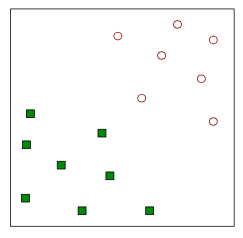
\includegraphics[width=0.9\textwidth]{img/Schermata 2024-06-12 alle 14.23.03.png}
    \caption*{(a) Find a linear hyperplane (decision boundary) that separates the data.}
  \end{minipage}
  \hfill
  \begin{minipage}[t]{0.3\textwidth}
    \centering
    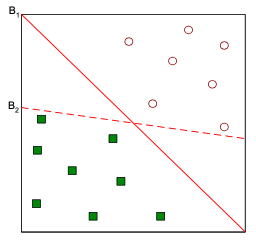
\includegraphics[width=0.95\textwidth]{img/Schermata 2024-06-12 alle 14.22.40.png}
    \caption*{(b) Possible solutions.}
  \end{minipage}
  \hfill
  \begin{minipage}[t]{0.3\textwidth}
    \centering
    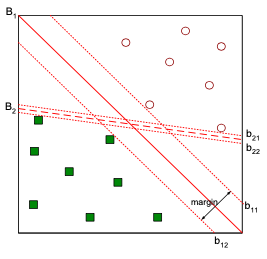
\includegraphics[width=0.98\textwidth]{img/Schermata 2024-06-12 alle 14.22.32.png}
    \caption*{(c) The best is the hyperplane that maximizes the margin, so $B_1$ is better than $B_2$.}
  \end{minipage}

  \caption{Different hyperplanes and their corresponding margins.}
\end{figure}

A \textbf{linear SVM} is a classifier that searches for a hyperplane with the largest margin (also called the maximal margin classifier).

\subsubsection{Optimal Hyperplane and Soft Margin SVM}
The decision boundaries are defined as $\vec{w} \cdot \vec{x} + b = k$, where $k \in \{-1,0,1\}$, and the closest data points are the support vectors.  
The classifier is defined as:
\begin{equation}
f(\vec{x}) = \begin{cases}
    1 & \text{if } \vec{w} \cdot \vec{x} + b \geq 1 \\
    -1 & \text{if } \vec{w} \cdot \vec{x} + b \leq -1
\end{cases}    
\end{equation}
The distance of a point $\vec{x}$ from the decision boundary $\vec{w} \cdot \vec{x} + b = 0$ is given by:
\begin{equation}
d(x) = \frac{| \vec{x} \cdot \vec{w} + b |}{||\vec{w}||_2} = \frac{| \vec{x} \cdot \vec{w} + b |}{\sqrt{\sum_{i=1}^d w_i^2}}    
\end{equation}

\paragraph{Optimize the Margin}
The margin, the distance between the two support vector boundaries, is $\frac{2}{||\vec{w}||}$.
Maximizing the margin is equivalent to minimizing $||\vec{w}||$, leading to the optimization problem:
\begin{align}
\min_{\vec{w}, b} \quad &L(\vec{w}) = \frac{1}{2} ||\vec{w}||^2\\
    \text{subject to } \quad&
y_i (\vec{w} \cdot \vec{x}_i + b) \geq 1, \quad \forall i = 1, \dots, N    
\end{align}

\paragraph{Dual Formulation}
We solve this constrained optimization problem with Lagrange multipliers:
\begin{equation}
L(\vec{w}, b, \lambda) = \frac{1}{2} ||\vec{w}||^2 - \sum_{i} \lambda_i [y_i (\vec{w} \cdot \vec{x}_i + b) - 1]    
\end{equation}
Setting the derivatives to zero and substituting back into $L$ yields the dual problem:
\begin{align}
\max_{\lambda} &\sum_i \lambda_i - \frac{1}{2} \sum_{i,j} y_i y_j \lambda_i \lambda_j \langle \vec{x}_i, \vec{x}_j \rangle\\
\text{subject to}& \sum_i \lambda_i y_i = 0, \quad \lambda_i \geq 0
\end{align}    

For non-linearly separable cases, we introduce \textbf{slack variables} $\xi_i$ to allow misclassification:
\begin{equation}
y_i (\vec{w} \cdot \vec{x}_i + b) \geq 1 - \xi_i, \quad \xi_i \geq 0    
\end{equation}
where $\xi_i$ measures the violation of the margin constraint.
\paragraph{Soft Margin SVM (Primal Form)}
\begin{align*}
\min_{\vec{w}, b, \xi} & \Psi(\vec{w}, \xi) = \frac{1}{2} ||\vec{w}||^2 + C \sum_{i=1}^N \xi_i\\
\text{subject to } & y_i (\vec{w} \cdot \vec{x}_i + b) \geq 1 - \xi_i, \quad \xi_i \geq 0, \quad \forall i = 1, \dots, N
\end{align*}
The \textbf{regularization hyperparameter} $C$ balances margin maximization against misclassification: a low $C$ allows more errors (underfitting), while a high $C$ enforces strict separation (overfitting).

\paragraph{Soft Margin SVM (Dual Form)}
\begin{align*}
    \max_{\lambda} & \sum_{i=1}^N \lambda_i - \frac{1}{2} \sum_{i=1}^N \sum_{j=1}^N \lambda_i \lambda_j y_i y_j \langle \vec{x}_i, \vec{x}_j \rangle\\
\text{subject to } & 0 \leq \lambda_i \leq C, \quad \sum_{i=1}^N \lambda_i y_i = 0
\end{align*}
The Kuhn-Tucker conditions refine the constraints:
\begin{equation}
\lambda_i [y_i (\vec{w} \cdot \vec{x}_i + b) + \xi_i - 1] = 0, \quad \mu_i \xi_i = 0    
\end{equation}
where $\mu_i$ are Lagrange multipliers enforcing $\xi_i \geq 0$. If $0 < \lambda_i < C$, then $\xi_i = 0$.  
Solving the dual problem yields $\vec{w}_o$ and $b_o$, determining the optimal hyperplane.


\subsection{Mapping to a High-Dimensional Space}
\href{https://en.wikipedia.org/wiki/Cover%27s_theorem#The_Theorem}{Cover's theorem states that non-linearly separable problems can become linearly separable when mapped to a higher-dimensional \textbf{feature space}}. This approach parallels linear basis expansion in linear models. We define a mapping function $\phi: \mathbb{R}^{m_0} \rightarrow \mathbb{R}^{m_1}$.

Finding an appropriate mapping function is challenging without prior knowledge. Moreover, using excessively high-dimensional feature spaces risks overfitting. With this mapping, we transform the original data: $x \mapsto \phi(x)$. The problem becomes finding a hyperplane in the new space with training set $TR = \{(\phi(x_i), d_i)\}$ and separator $g(x) = w^T \phi(x) + b = 0$. For simplicity, we incorporate the bias into the weight vector by setting $w_0 = b$ and $\phi_0(x) = 1$:
\begin{align}
\phi(x) &= (1, \phi_1(x), \ldots, \phi_{m_1}(x))^T &[\text{Feature mapping with bias}]\\
w &= \sum_{i=1}^N \lambda_i d_i \phi(x_i) &[\text{Optimal weight vector}]\\
g(x) &= \sum_{i=1}^N \lambda_i d_i \phi^T(x_i) \phi(x) = 0 & [\text{Hyperplane equation}]
\end{align}

Direct computation of $\phi(x)$ may be computationally prohibitive. SVMs solve this through the \textbf{kernel trick}, which computes dot products in feature space without explicitly calculating the feature vectors. This is achieved using \textbf{kernel functions} $k: \mathbb{R}^{m_0} \times \mathbb{R}^{m_0} \rightarrow \mathbb{R}$ that compute inner products in the feature space. These symmetric functions satisfy $k(x_i, x) = k(x, x_i)$.

\paragraph{Polynomial Kernel Behaviour}
    The \textbf{Polynomial Kernel} has a parameter $d$, the \textit{degree} of the polynomial. The degree $d$ controls the order of feature interactions the kernel captures: $d=1$ keeps only first-order (linear) terms, while $d=2$ adds all pairwise products of the input features (quadratic terms), and larger $d$ adds higher-order monomials. The implicit feature-space dimension grows combinatorially with $d$. We pick the optimal value of $d$ by \textit{cross-validation}.

\begin{example}[Kernel computing]
Given $\phi(x) = \phi((x_1, x_2)^T) = (x_1^2, \sqrt{2}x_1x_2, x_2^2)^T$, $x = (x_1, x_2)^T$ and $y = (y_1, y_2)^T$ in $\mathbb{R}^2$:
\begin{align*}
    \phi^T(x)\phi(y) &= (x_1^2, \sqrt{2}x_1x_2, x_2^2) \cdot (y_1^2, \sqrt{2}y_1y_2, y_2^2)^T \\
    &= x_1^2y_1^2 + 2x_1y_1x_2y_2 + x_2^2y_2^2 = (x_1y_1 + x_2y_2)^2 \\
    &= (x^Ty)^2 = k(x, y)
\end{align*}
\end{example}

We can organize the dot products in feature space between training patterns in a \textbf{kernel matrix}:
\begin{equation*}
    K = \begin{pmatrix}
        k(x_1,x_1) & \cdots & k(x_1, x_N) \\
        \vdots & & \vdots \\
        k(x_N,x_1) & \cdots & k(x_N, x_N) \\
        \end{pmatrix} = \{k(x_i, x_j)\}_{i,j=1}^N
\end{equation*}

The kernel matrix is symmetric. Not all functions qualify as valid kernels; \href{https://en.wikipedia.org/wiki/Mercer%27s_theorem}{only those producing positive semi-definite matrices with non-negative eigenvalues can be used as kernels}.

Given kernels $k_1$ and $k_2$ over $\mathbb{R}^{m_0} \times \mathbb{R}^{m_0}$, the following are also valid kernels:
\begin{itemize}
    \item $k_1(x,y) + k_2(x,y)$
    \item $\lambda k_1(x,y)$ for all $\lambda \in \mathbb{R}_+$
    \item $k_1(x,y)k_2(x,y)$
\end{itemize}

\paragraph{Quadratic Optimization in Feature Space (Primal Form)}
Given $TR = < \phi(x_i),d_i >$, find $w$ solving:
\begin{align*} \min_{w, \xi} \quad & \Psi(w, \xi) = \frac{1}{2}w^T w + C \sum_{i=1}^N \xi_i \\
\text{subject to} \quad & d_i (w^T \phi(x_i)) \geq 1 - \xi_i,\quad \xi_i \geq 0, \quad \forall i = 1, \dots, N \end{align*}

\paragraph{Quadratic Optimization in Feature Space (Dual Form)} Given $TR = < \phi(x_i),d_i >$, find $\lambda_i$ solving:
\begin{align*} \max_{\lambda} \quad & Q(\lambda) = \sum_{i=1}^N \lambda_i - \frac{1}{2} \sum_{i,j=1}^N \lambda_i \lambda_j d_i d_j k(x_i,x_j) \\ \text{subject to} \quad& \sum_{i=1}^N \lambda_i d_i = 0 \quad 0 \leq \lambda_i \leq C, \quad \forall i = 1, \dots, N \end{align*}

To classify a new input pattern $x$, we compute $\sum_{i=1}^N \lambda_i d_i k(x, x_i)$ and classify $x$ as $h(x) = \text{sign}\left(\sum_{i=1}^N \lambda_i d_i k(x, x_i)\right)$. Note that we must store the training examples $x_i$ for the testing phase.

\subsubsection{Commonly Used Kernel Functions}
\begin{itemize}
    \item \textbf{Polynomial Learning Machine}: $k(x, x_i) = (x^T x_i + 1)^p$ where $p$ is a user-specified parameter
    \item \textbf{Radial Basis Function (RBF)}: $k(x, x_i) = \exp\left(-\frac{\|x - x_i\|^2}{2\sigma^2}\right)$ where $\sigma$ is a user-specified parameter. This behaves like a weighted Nearest Neighbor model, where closer observations have greater impact on classification.
    \item \textbf{Two-layer Perceptron}: $k(x, x_i) = \tanh(\beta_0 x^T x_i + \beta_1)$ where $\beta_0 > 0$ and $\beta_1 < 0$ are user-specified parameters.
\end{itemize}

Using an RBF kernel always maps to a feature space with an infinite number of dimensions.


\subsection{Multiclass Classification Methods}

Multiclass classification extends binary classification to more than two classes. We cover two families: adapting binary classifiers by decomposition, and a specialized SVM formulation that trains one multiclass model directly.

Binary classifiers reach multiclass problems through two decomposition strategies: \textbf{One-versus-all} and \textbf{All-versus-all}.

\subsubsection{One-Versus-All Classification}
\textbf{One-versus-all} assumes each class can be separated from all others combined. Given dataset $D = \{(\mathbf{x}_i, y_i)\}$, where $\mathbf{x}_i \in \mathbb{R}^n$ and $y_i \in \{1, 2, \ldots, K\}$, we create $K$ binary tasks. For each class $k$, examples with label $k$ become positive, while all others become negative.

This creates $K$ binary classifiers with weight vectors $\mathbf{w}_1, \mathbf{w}_2, \ldots, \mathbf{w}_K$. For prediction, we use "Winner Takes All":

\begin{equation}
\text{predicted class} = \arg\max_i \mathbf{w}_i^T\mathbf{x}
\end{equation}

With three classes (blue, red, green), we train three classifiers: $\mathbf{w}_{\text{blue}}^T\mathbf{x} > 0$ identifies blue inputs, $\mathbf{w}_{\text{red}}^T\mathbf{x} > 0$ identifies red inputs, and $\mathbf{w}_{\text{green}}^T\mathbf{x} > 0$ identifies green inputs.

This approach fails when a class is not linearly separable from all the others combined. It also lacks strong theoretical justification and faces calibration problems, since the scores come from classifiers trained independently. Even so, One-versus-all works well in many practical settings once properly tuned.

\subsubsection{All-Versus-All Classification}

\textbf{All-versus-all} assumes every pair of classes is separable. For dataset $D = \{(\mathbf{x}_i, y_i)\}$, we create a binary classifier for every class pair $(j, k)$. Examples with label $j$ become positive, those with label $k$ become negative, and others are ignored.

This requires $\binom{K}{2} = \frac{K(K-1)}{2}$ binary classifiers. For prediction, each label receives $K-1$ votes, with classification determined by majority voting or tournament methods.

\begin{equation}
\text{Total classifiers} = \frac{K(K-1)}{2}
\end{equation}

While effective when class pairs are linearly separable, this approach has limitations: it requires $O(K^2)$ weight vectors, risks overfitting with small training sets for each pair, and uses potentially unstable ad-hoc prediction methods.

\subsubsection{Multiclass SVM}
Decomposition methods don't optimize for global correctness. This limitation motivates developing approaches that directly train a single multiclass classifier.

\textbf{Multiclass SVM} extends binary SVM concepts to handle multiple classes directly. While binary SVMs maximize margin by minimizing weight norm such that the closest points score at least $\pm 1$, Multiclass SVM assigns each label a different weight vector.

The objective becomes maximizing the multiclass margin, equivalent to minimizing total weight norm such that the true label's score exceeds any competing label's score by at least 1.

Mathematically, we learn weight vectors $\mathbf{w}_1, \mathbf{w}_2, \ldots, \mathbf{w}_K$ such that for each training example $(\mathbf{x}_i, y_i)$:

\begin{equation}
\mathbf{w}_{y_i}^T\mathbf{x}_i - \mathbf{w}_j^T\mathbf{x}_i \geq 1 - \xi_i, \quad \forall j \neq y_i
\end{equation}

where $\xi_i$ are slack variables allowing soft margins. The objective function minimizes the sum of all weight vector norms plus a penalty term for the slack variables, so the $K$ weight vectors are trained jointly rather than one at a time.

\subsection{Advantages and Limitations}
\begin{footnotesize}
\begin{tabular}{p{0.47\textwidth} | p{0.47\textwidth}}
\toprule
\textbf{Advantages} & \textbf{Limitations} \\
\midrule
\midrule
\begin{itemize}[leftmargin=*,nosep]
    \item Built-in regularization without extra hyperparameters
    \item Approximates Structural Risk Minimization by optimizing VC-dimension
    \item Guarantees global minimum (convex optimization)
    \item Enables implicit feature transformation through kernels
    \item Maintains linear model complexity bounded by margin
    \item Supports rich non-linear functions via kernel methods
\end{itemize} &
\begin{itemize}[leftmargin=*,nosep]
    \item Requires manual kernel selection and parameterization
    \item Batch processing limits parallelization potential
    \item Scaling challenges with large datasets (despite optimizations)
    \item Soft margin parameter $C$ and kernel choice affect performance without theoretical guarantees
\end{itemize}\\
\bottomrule
\end{tabular}
\end{footnotesize}

\textbf{Note on Soft Margin SVM:} The VC-dimension varies with margin width: minimal margins (few support vectors) can fit arbitrarily large training sets but risk infinite VC-dimension, while large margins (most points as support vectors) reduce VC-dimension. This relationship resembles $k$-NN behavior: $k=1$ (high variance) vs. $k=l$ (high bias). Cross-validation for tuning $C$ and kernel parameters remains essential.